\documentclass[11pt]{article}
\usepackage[top=20mm,bottom=30mm,left=20mm,right=20mm]{geometry}
\usepackage[utf8]{inputenc}
\usepackage{parskip}

% Mathy stuff
\usepackage{physics}
\usepackage{siunitx}
\usepackage{amsmath}
\usepackage[version=4]{mhchem}

% Visual stuff
\usepackage{graphics}
\usepackage{tikz}
\usetikzlibrary{math}
\usepackage{stackengine}
\usepackage{float}
\usepackage{tcolorbox}

% Misc
\usepackage{subcaption}
\usepackage{cleveref}
\usepackage{lipsum}

\allowdisplaybreaks

\setlength{\parskip}{2ex}
\setlength{\parindent}{0em}

\newcommand\set[1]{\ensuremath{\{#1\}}}
\newcommand\textbff[1]{\textbf{\boldmath #1}}
\newcommand{\shortnote}[1]{\textit{\footnotesize (#1)}}

\stackMath
\newcommand{\suf}[2]{\stackunder[0.5pt]{\stackunder[1pt]{\ensuremath{#1}}{\rule{\widthof{\ensuremath{#2}}*\real{0.9}}{.1ex}}}{}}
\newcommand{\duf}[2]{\stackunder[0.5pt]{\stackunder[0.8pt]{\stackunder[1pt]{\ensuremath{#1}}{\rule{\widthof{\ensuremath{#2}}*\real{0.9}}{.1ex}}}{\rule{\widthof{\ensuremath{#2}}*\real{0.9}}{.1ex}}}{}}
\newcommand{\su}[1]{\suf{#1}{#1}}
\newcommand{\du}[1]{\duf{#1}{#1}}
\newcommand{\ssu}[1]{\scriptsize\su{#1}\normalsize}
\newcommand{\sdu}[1]{\scriptsize\du{#1}\normalsize}

\newcommand{\pp}{\ensuremath{\partial}}

\tikzmath{
    \D = 2;
}

\begin{document}
\begin{center}
    \LARGE
    \textbf{Ones}
    \vspace{1em}
\end{center}

\section{Two Digit Cycles}
What are all the different (as in they lead to different behaviours) 2 digit cycles we can implement in the model?
In the diagrams as shown in \cref{fig:2d4s} we first note that the diagrams lead to the same behaviour if they are the same under reflection along the top-left to bottom-right axis which corresponds to reflecting the sequence (physically the same system if working with a loop geometry).
We first focus on such cycles that visit all possible 2 digit sequences.
We either get diagrams with or without a crossing, and there is only one diagram without a crossing which is \cref{fig:2d4ss}.
For diagrams with a crossing that visit all four 2 digit sequences we always the motif as in \cref{fig:2d4sc1,fig:2d4sc2} which are the only such diagrams up to the mentioned reflection.
Also note that the two cycles with crossings are reverses of each other!

\begin{figure}[H]
    \centering
    \begin{subfigure}[t]{0.3\textwidth}
        \centering
        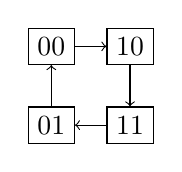
\begin{tikzpicture}
            \node[draw] (a) at (0,\D) {00};
            \node[draw] (b) at (\D,\D) {10};
            \node[draw] (c) at (\D,0) {11};
            \node[draw] (d) at (0,0) {01};

            \draw[->] (a) -- (b);
            \draw[->] (b) -- (c);
            \draw[->] (c) -- (d);
            \draw[->] (d) -- (a);
        \end{tikzpicture}
        \caption{simple}\label{fig:2d4ss}
    \end{subfigure}
    \begin{subfigure}[t]{0.3\textwidth}
        \centering
        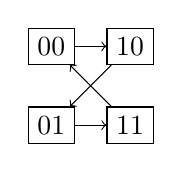
\begin{tikzpicture}
            \node[draw] (a) at (0,\D) {00};
            \node[draw] (b) at (\D,\D) {10};
            \node[draw] (c) at (\D,0) {11};
            \node[draw] (d) at (0,0) {01};

            \draw[->] (a) -- (b);
            \draw[->] (b) -- (d);
            \draw[->] (d) -- (c);
            \draw[->] (c) -- (a);
        \end{tikzpicture}
        \caption{crossing with $00\rightarrow10$}\label{fig:2d4sc1}
    \end{subfigure}
    \begin{subfigure}[t]{0.3\textwidth}
        \centering
        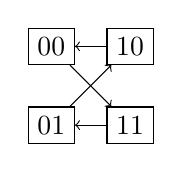
\begin{tikzpicture}
            \node[draw] (a) at (0,\D) {00};
            \node[draw] (b) at (\D,\D) {10};
            \node[draw] (c) at (\D,0) {11};
            \node[draw] (d) at (0,0) {01};

            \draw[->] (a) -- (c);
            \draw[->] (c) -- (d);
            \draw[->] (d) -- (b);
            \draw[->] (b) -- (a);
        \end{tikzpicture}
        \caption{crossing with $00\rightarrow11$}\label{fig:2d4sc2}
    \end{subfigure}
    \caption{
        All the different 2 digit simple cycles that visit all four such sequences, these are unique up to right-left reflection.
    }\label{fig:2d4s}
\end{figure}

Following the same logic, we only get four cycles which visit 3 of the sequences, shown in \cref{fig:2d3s}.
With the last two also being reveres of each other.
We don't examine cycles which visit only 2 of the sequences as it's difficult to imagine anything interesting taking place.

\begin{figure}[H]
    \centering
    \begin{subfigure}[t]{0.2\textwidth}
        \centering
        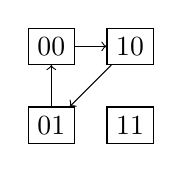
\begin{tikzpicture}
            \node[draw] (a) at (0,\D) {00};
            \node[draw] (b) at (\D,\D) {10};
            \node[draw] (c) at (\D,0) {11};
            \node[draw] (d) at (0,0) {01};

            \draw[->] (a) -- (b);
            \draw[->] (b) -- (d);
            \draw[->] (d) -- (a);
        \end{tikzpicture}
        \caption{}
    \end{subfigure}
    \begin{subfigure}[t]{0.2\textwidth}
        \centering
        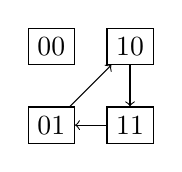
\begin{tikzpicture}
            \node[draw] (a) at (0,\D) {00};
            \node[draw] (b) at (\D,\D) {10};
            \node[draw] (c) at (\D,0) {11};
            \node[draw] (d) at (0,0) {01};

            \draw[->] (d) -- (b);
            \draw[->] (b) -- (c);
            \draw[->] (c) -- (d);
        \end{tikzpicture}
        \caption{}
    \end{subfigure}
    \begin{subfigure}[t]{0.2\textwidth}
        \centering
        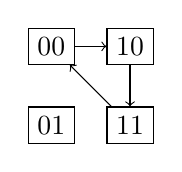
\begin{tikzpicture}
            \node[draw] (a) at (0,\D) {00};
            \node[draw] (b) at (\D,\D) {10};
            \node[draw] (c) at (\D,0) {11};
            \node[draw] (d) at (0,0) {01};

            \draw[->] (a) -- (b);
            \draw[->] (b) -- (c);
            \draw[->] (c) -- (a);
        \end{tikzpicture}
        \caption{}
    \end{subfigure}
    \begin{subfigure}[t]{0.2\textwidth}
        \centering
        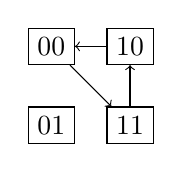
\begin{tikzpicture}
            \node[draw] (a) at (0,\D) {00};
            \node[draw] (b) at (\D,\D) {10};
            \node[draw] (c) at (\D,0) {11};
            \node[draw] (d) at (0,0) {01};

            \draw[->] (b) -- (a);
            \draw[->] (c) -- (b);
            \draw[->] (a) -- (c);
        \end{tikzpicture}
        \caption{}
    \end{subfigure}
    \caption{
        All the different 2 digit simple cycles that do not visit all such sequences, these are unique up to right-left reflection.
    }\label{fig:2d3s}
\end{figure}

As reverses of cycles will give exactly the same behaviour just revered in time, we can focus on only one of each such cycles.
In addition, it is reasonable to suspect that replacing all 0s by 1s and vice versa should also be some symmetry of the system and so we only look at one cycle for each of such classes.
This gives only the cycles shown in \cref{fig:2dint} to look at.

Of these of most interest is the first as that is the only one which does not change two digits at once, a perhaps reasonable physical constraint.
\Cref{fig:2dbase_graphs} shows the resulting graphs for a couple of different $N$, where we get very interesting loop patterns, though the steady states are still always uniform!

\begin{tcolorbox}
    \begin{figure}[H]
        \centering
        \begin{subfigure}[t]{0.2\textwidth}
            \centering
            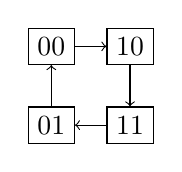
\begin{tikzpicture}
                \node[draw] (a) at (0,\D) {00};
                \node[draw] (b) at (\D,\D) {10};
                \node[draw] (c) at (\D,0) {11};
                \node[draw] (d) at (0,0) {01};

                \draw[->] (a) -- (b);
                \draw[->] (b) -- (c);
                \draw[->] (c) -- (d);
                \draw[->] (d) -- (a);
            \end{tikzpicture}
            \caption{}\label{fig:2dbase}
        \end{subfigure}
        \begin{subfigure}[t]{0.2\textwidth}
            \centering
            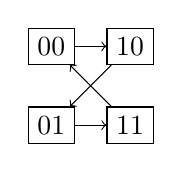
\begin{tikzpicture}
                \node[draw] (a) at (0,\D) {00};
                \node[draw] (b) at (\D,\D) {10};
                \node[draw] (c) at (\D,0) {11};
                \node[draw] (d) at (0,0) {01};

                \draw[->] (a) -- (b);
                \draw[->] (b) -- (d);
                \draw[->] (d) -- (c);
                \draw[->] (c) -- (a);
            \end{tikzpicture}
            \caption{}
        \end{subfigure}
        \begin{subfigure}[t]{0.2\textwidth}
            \centering
            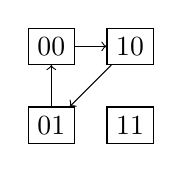
\begin{tikzpicture}
                \node[draw] (a) at (0,\D) {00};
                \node[draw] (b) at (\D,\D) {10};
                \node[draw] (c) at (\D,0) {11};
                \node[draw] (d) at (0,0) {01};

                \draw[->] (a) -- (b);
                \draw[->] (b) -- (d);
                \draw[->] (d) -- (a);
            \end{tikzpicture}
            \caption{}
        \end{subfigure}
        \begin{subfigure}[t]{0.2\textwidth}
            \centering
            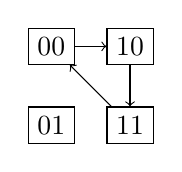
\begin{tikzpicture}
                \node[draw] (a) at (0,\D) {00};
                \node[draw] (b) at (\D,\D) {10};
                \node[draw] (c) at (\D,0) {11};
                \node[draw] (d) at (0,0) {01};

                \draw[->] (a) -- (b);
                \draw[->] (b) -- (c);
                \draw[->] (c) -- (a);
            \end{tikzpicture}
            \caption{}
        \end{subfigure}
        \caption{
            The only 2 digit simple cycles that are worth investigating.
            Of which only the first only affects 1 digit at a time -- thus this is the main object of interest.
        }\label{fig:2dint}
    \end{figure}
\end{tcolorbox}

\begin{tcolorbox}
    \begin{figure}[H]
        \centering
        \begin{subfigure}[t]{0.49\textwidth}
            \centering
            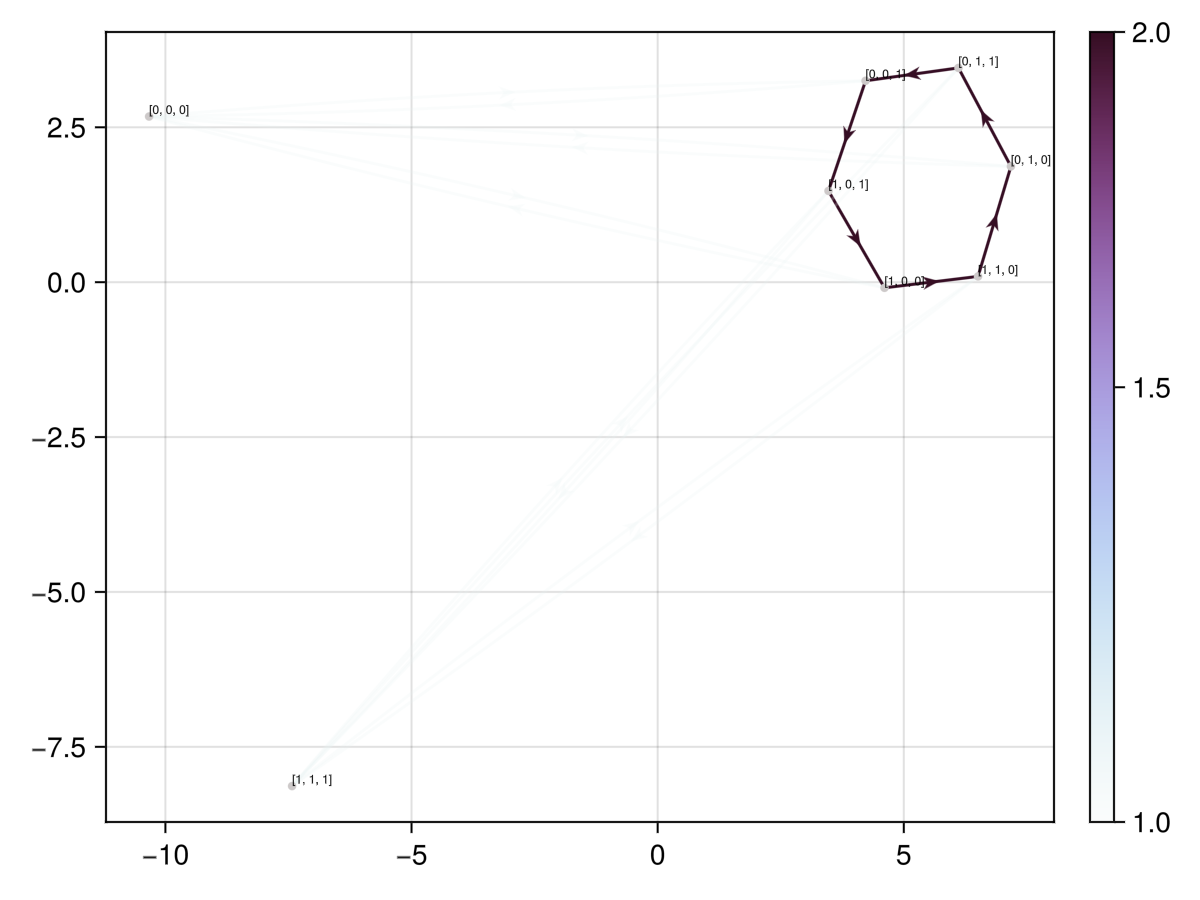
\includegraphics[width=\textwidth]{../../plots/ones/c1/spring_N=3_metadata=(chash=5795298381321907906,ctype=simple).png}
            \caption{$N=3$}
        \end{subfigure}
        \begin{subfigure}[t]{0.49\textwidth}
            \centering
            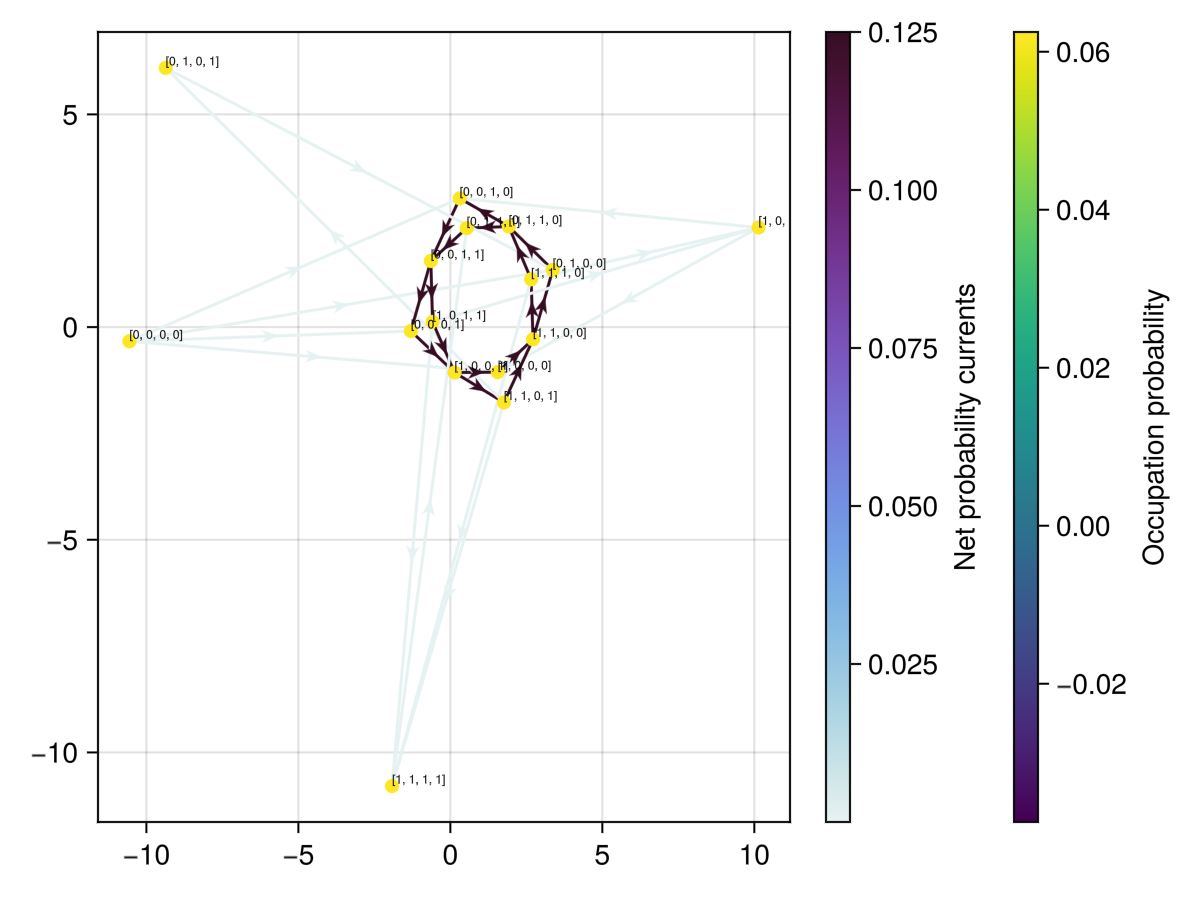
\includegraphics[width=\textwidth]{../../plots/ones/c1/spring_N=4_metadata=(chash=5795298381321907906,ctype=simple).png}
            \caption{$N=4$}
        \end{subfigure}
        \begin{subfigure}[t]{0.49\textwidth}
            \centering
            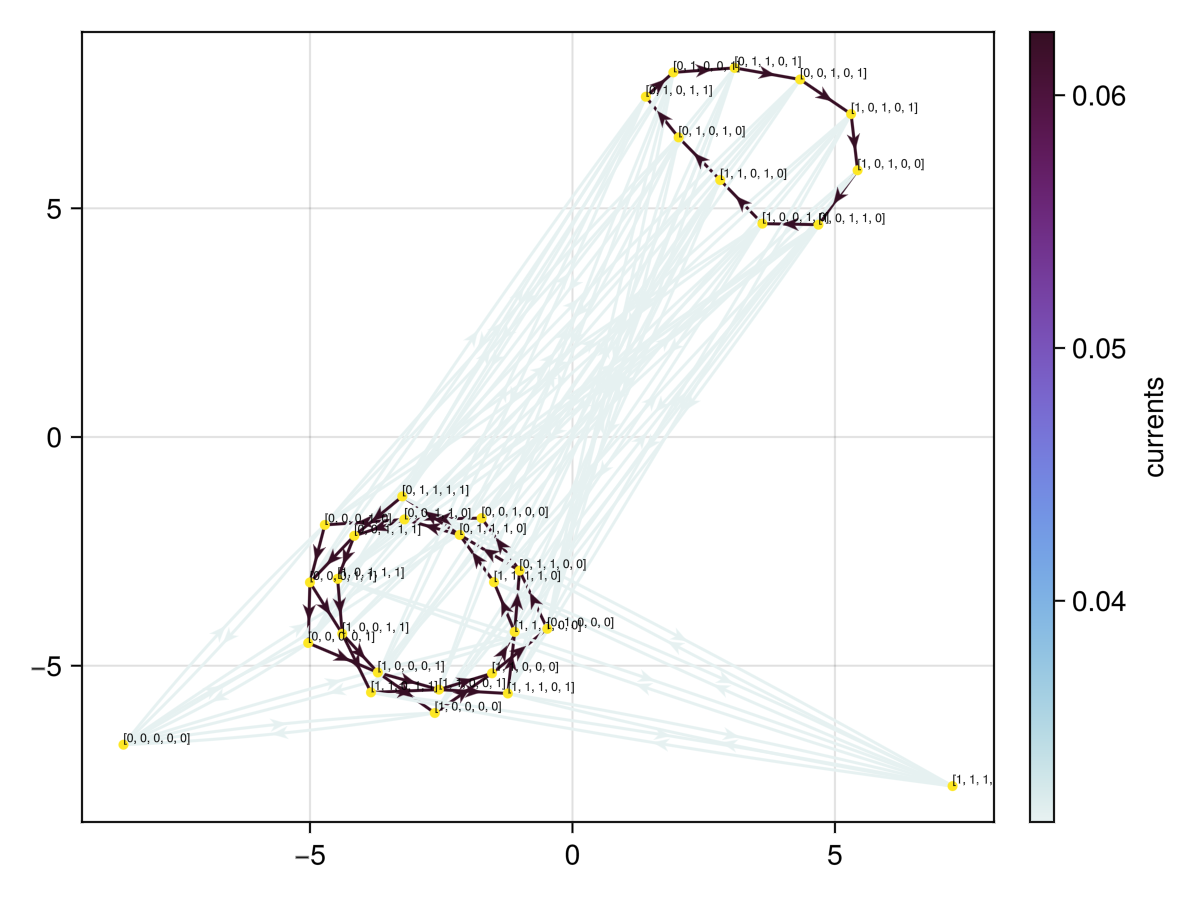
\includegraphics[width=\textwidth]{../../plots/ones/c1/spring_N=5_metadata=(chash=5795298381321907906,ctype=simple).png}
            \caption{$N=5$}
        \end{subfigure}
        \begin{subfigure}[t]{0.49\textwidth}
            \centering
            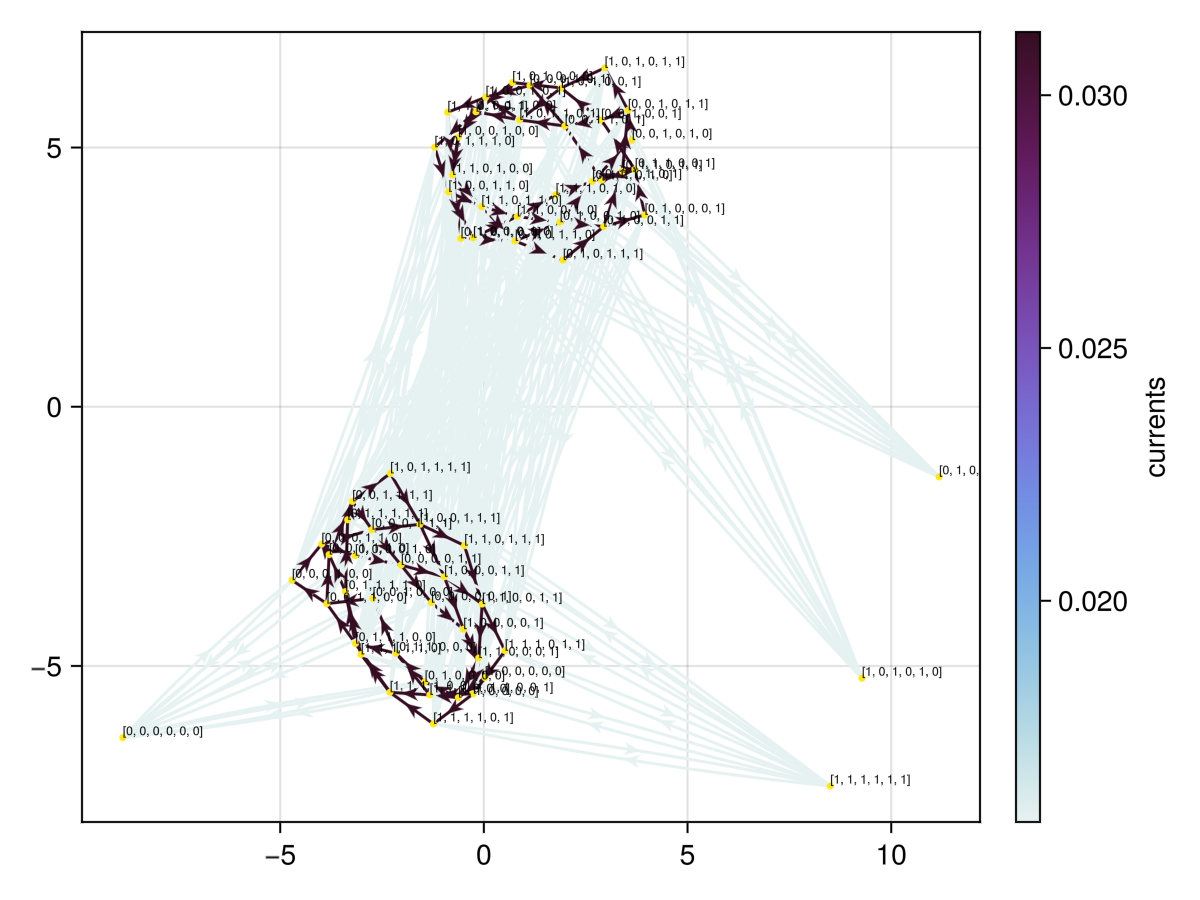
\includegraphics[width=\textwidth]{../../plots/ones/c1/spring_N=6_metadata=(chash=5795298381321907906,ctype=simple).png}
            \caption{$N=6$}
        \end{subfigure}
        \caption{
            Resulting transition graphs when using only the cycle from \cref{fig:2dbase} for different $N$ in the loop geometry.
            The node color shows the steady state probability of that node, which notably is always uniform!
            Transition colors designate the probability current.
        }\label{fig:2dbase_graphs}
    \end{figure}
\end{tcolorbox}

The other base cycles all give rise to not quite as interesting patterns, some of which are shown in  .
And it is also worth noting that all of these also gave rise only to uniform steady states.

\begin{figure}[H]
    \centering
    \begin{subfigure}[t]{0.49\textwidth}
        \centering
        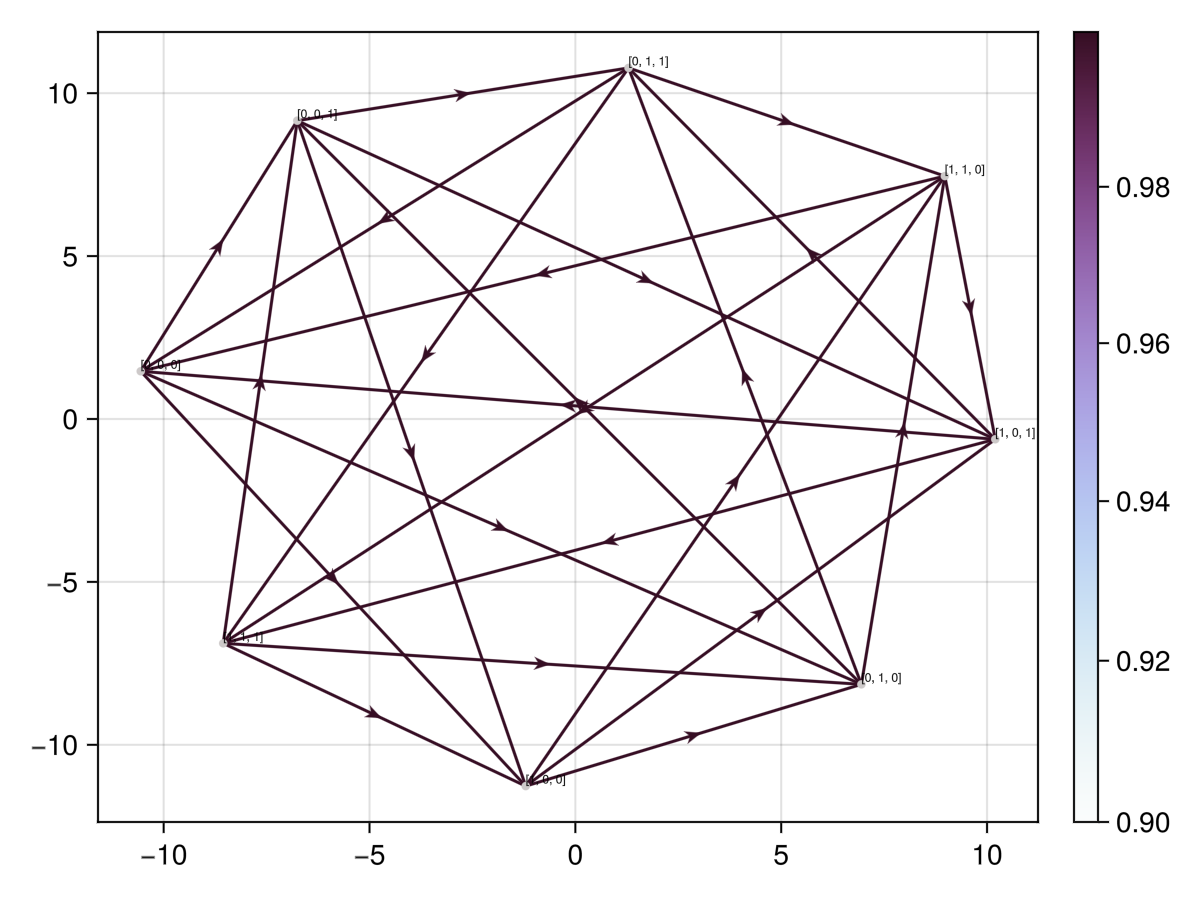
\includegraphics[width=\textwidth]{../../plots/ones/c2/spring_N=3_metadata=(chash=835941404624685282,ctype=simple).png}
        \caption{Second cycle, $N=3$}
    \end{subfigure}
    \begin{subfigure}[t]{0.49\textwidth}
        \centering
        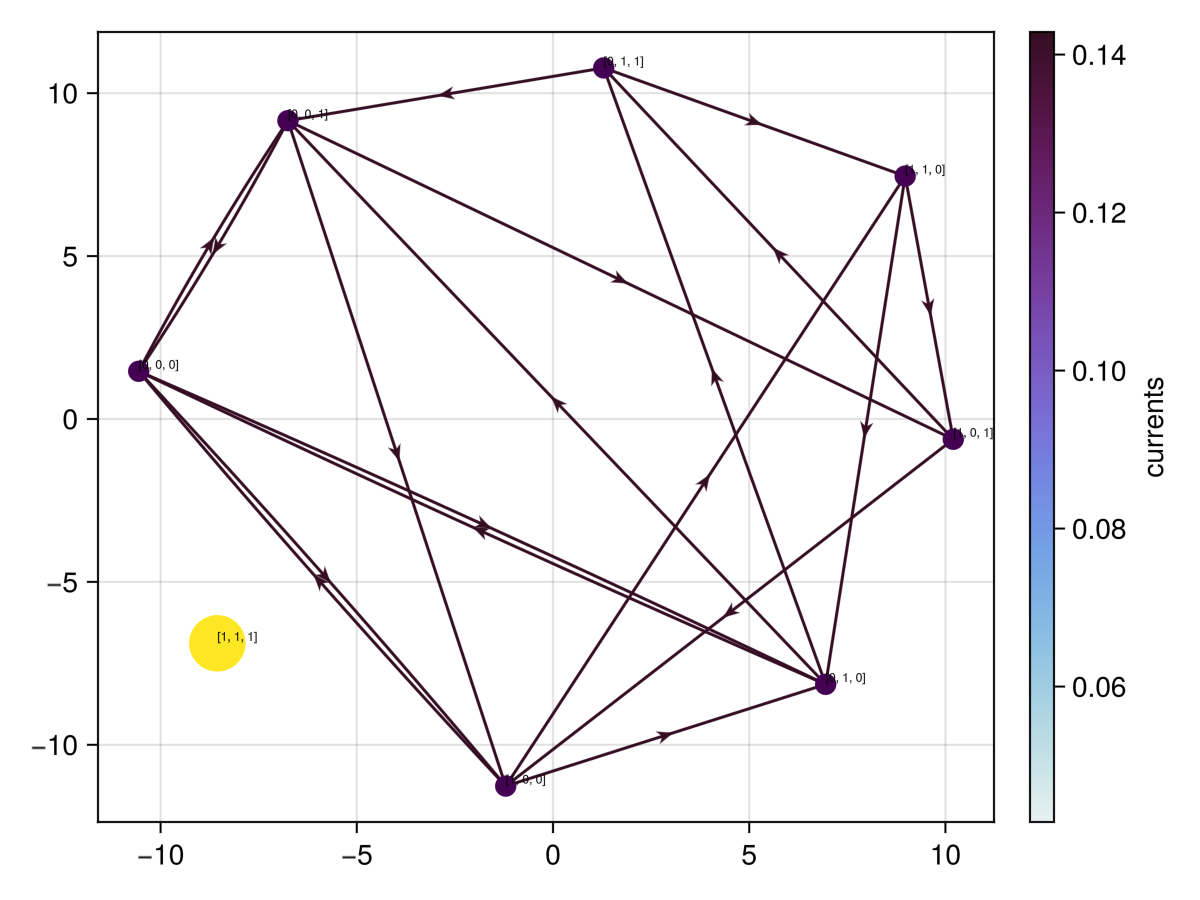
\includegraphics[width=\textwidth]{../../plots/ones/c3/spring_N=3_metadata=(chash=14397644121192019449,ctype=simple).png}
        \caption{Third cycle, $N=3$}
    \end{subfigure}
    \begin{subfigure}[t]{0.49\textwidth}
        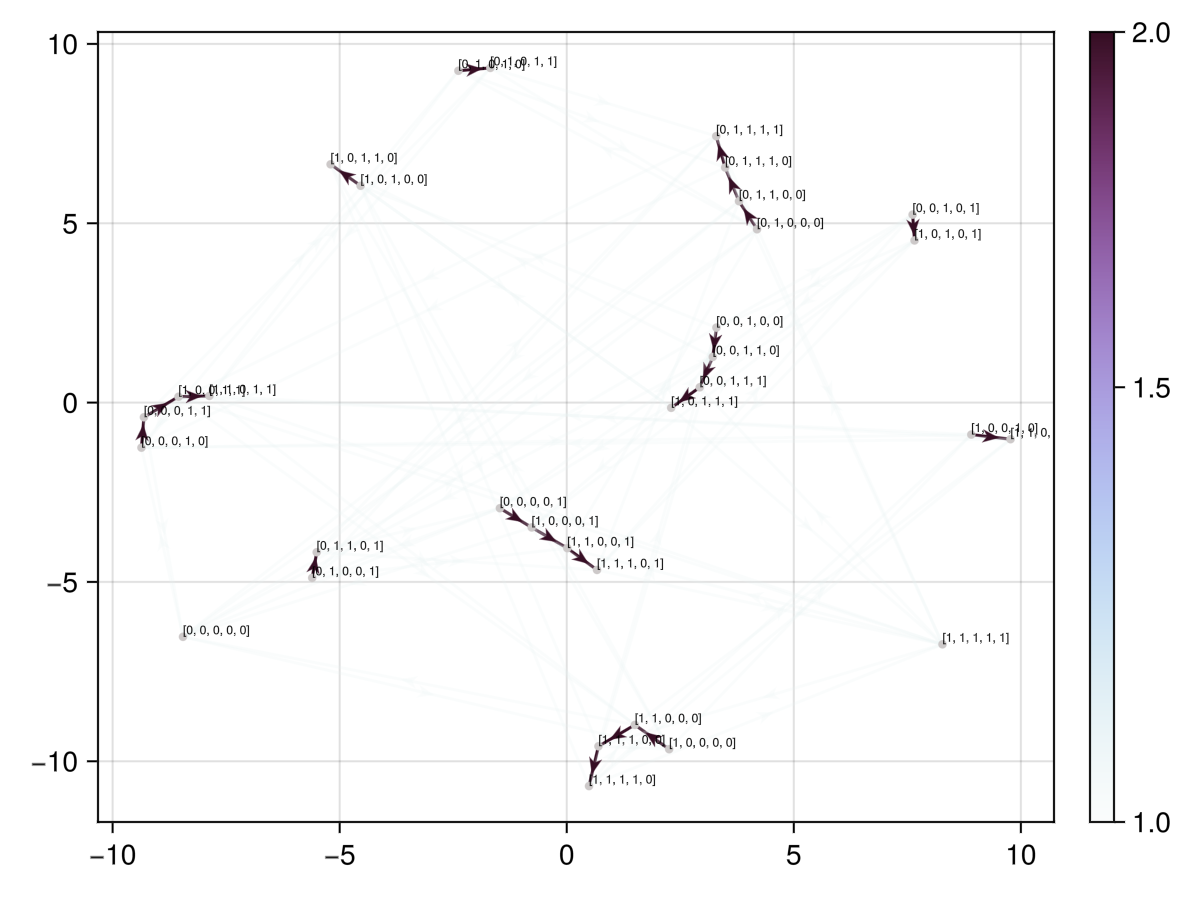
\includegraphics[width=\textwidth]{../../plots/ones/c4/spring_N=5_metadata=(chash=2008083833646787391,ctype=simple).png}
        \centering
        \caption{Fourth cycle, $N=3$}
    \end{subfigure}
    \begin{subfigure}[t]{0.49\textwidth}
        \centering
        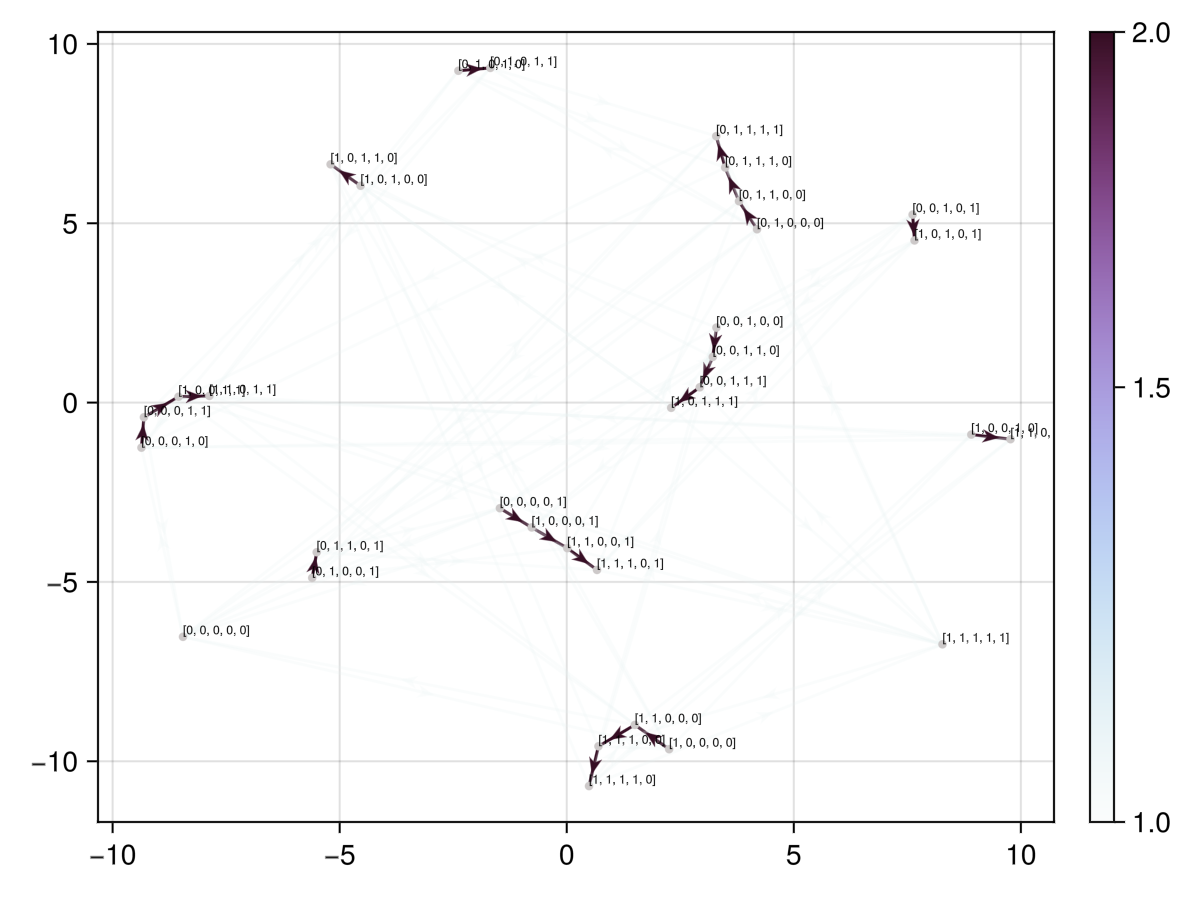
\includegraphics[width=\textwidth]{../../plots/ones/c4/spring_N=5_metadata=(chash=2008083833646787391,ctype=simple).png}
        \caption{Fourth cycle, $N=5$}
    \end{subfigure}
    \caption{
        Some example transition graphs for the other 2 digit base cycles from \cref{fig:2dint}.
    }\label{fig:2dothers}
\end{figure}

\end{document}
